\chapter{Task Scheduling with Provenance Support in Multisite Clouds} \label{SWSPSMC}

Recently, some Scientific Workflow Management Systems (SWfMSs) with provenance support (\textit{e.g.} Chiron) have been deployed in the cloud.
However,  they typically use a single cloud site. In this chapter, we consider a multisite cloud, where the data and computing resources are distributed at different sites (possibly in different regions).
Based on a multisite architecture of SWfMS, \textit{i.e.} multisite Chiron, and its provenance model, we propose a multisite task scheduling algorithm that considers the time to generate provenance data. This thesis is based on \cite{Liu2016}.

Section \ref{sec:FGPD} presents the problems for task scheduling of SWf execution in a multisite cloud environment. 
Then, Section \ref{sec:FGSA} gives the design of a multisite SWfMS. 
Afterwards, Section \ref{sec:FGTS} explains our proposed scheduling algorithm. 
Section \ref{sec:FGVal} gives our our extensive experimental evaluation of the algorithm using Microsoft Azure
multisite cloud and two real-life scientific workflows (Buzz and Montage). 
The results show that our scheduling algorithm is much better than baseline algorithms in terms of execution time and the amounts of intersite transferred data.

\section{Proposal Overview and Motivations}

SWfs are generally used to model the data processing of large scale \textit{in silico} scientific experiments as a graph, in which vertices represent data processing activities and edges represent dependencies between them. 
Since SWf activities may process multiple data chunks, one activity can correspond to several executable tasks for different parts of input data during SWf execution.
Thus, efficiently executing data-intensive SWfs, \textit{e.g.} Montage \cite{Montage} and Buzz \cite{Dias2013}, becomes an important issue. 

Some implementations of SWfMSs are publicly available, \textit{e.g.} Pegasus  \cite{Deelman2005} and Chiron \cite{Ogasawara2013}. 
A SWfMS generally supports provenance data, which is the metadata that captures the derivation history of a dataset \cite{Liu2015}, during SWf execution.
Provenance data, which is used for SWf analysis and SWf reproducibility, may be as important as the scientifc experiment itself \cite{Liu2015}. The provenance data is typically stored in a database to provide on-line provenance query \cite{Mattoso2014}, and contains the information regarding activities, tasks and files. During the execution of a task, there may be multiple exchanges of provenance data between the computing node and the provenance database. 


Recently, some SWfMSs with provenance support (\textit{e.g.} Chiron) have been deployed in the cloud.
However,  they typically focus the execution of a SWf at a single cloud site or in even a single computing node \cite{Hiden2010}\cite{Hiden2012}. Although there are some multisite solutions \cite{Duan2014}\cite{Luis2015}, they do not support provenance data, which is important for the analysis of SWf execution.
However, the data and computing resources (including programs) necessary to run a SWf
may well be distributed at different sites (possibly in different regions), \textit{e.g.} because of collaboration between different groups of scientists.
And it may not be always possible to move all the resources to a single site for execution.
Chapter \ref{MOSSWMC} focuses on the scheduling of fragments, which is coarse-grained and cannot address the problem of executing an activities at multiple sites.
In this chapter, we consider a multisite cloud that is composed of several sites (or data centers) of the same cloud provider, each with its own resources and data for the execution of each activity. In addition, we also take into consideration of the influence of the functionality of provenance data on the SWf multisite execution.

To enable SWf execution in a multisite cloud with distributed input data, the execution
of the tasks of each activity should be scheduled to a corresponding cloud site (or site for short). Then, the scheduling problem is to decide at which sites to execute the tasks in order to achieve a given objective, \textit{e.g.} reducing execution time. 
Compared with the approach of scheduling activities at a single site \cite{Liu2014}, the task scheduling is fine-grained, which enables the execution of the same activity at different sites to deal with distributed data and programs.
Furthermore, since it may take much time to transfer data between two different sites, the multisite scheduling problem should take into account the resources at different sites, \textit{e.g.} different bandwidths.

We focus on the task scheduling problem to reduce the makespan, \textit{i.e.} the execution time, of executing a SWf in a multisite cloud.
We use a distributed SWfMS architecture with a master site that coordinates the execution of each site and that stores all the provenance data of SWf execution.
In this architecture, the intersite transferred data can be intermediate data or provenance data produced by SWf execution. The intermediate data is the data generated by executing activities and can also be the input data for the tasks of following activities. 
In the multisite cloud, the bandwidth between two different sites (of different regions) may be small.
For data-intensive SWfs, there may be many data, \textit{e.g.} intermediate data and provenance data, to transfer across different sites for the execution of a task while the time to execute the task can be very small, \textit{e.g.} a few seconds or even less than one second.
As a result, the time to transfer intermediate data and the time to generate the provenance data connot be ignored in the scheduling process. Thus, we also consider the time to transfer both the intermediate data and the provenance data in the scheduling process in order to better reduce the overall execution time of SWf execution.

We make the following contributions. First, we propose multisite Chiron, with a novel architecture to execute SWfs in a multisite cloud environment while generating provenance data. 
Second, an extended multisite provenance model and global provenance management of distributed provenance data in multisite cloud.
Third, we propose a novel multisite task scheduling algorithm, \textit{i.e.} Data-Intensive Multisite task scheduling (DIM), for SWf execution with provenance support in multisite Chiron.
Fourth, we make an extensive experimental evaluation, based on the implementation of multisite Chiron in Microsoft Azure, and using two real SWf use cases (Buzz and Montage).


\section{Related Work}
\label{sec:FGrw}

Classic scheduling algorithms, \textit{e.g.} Opportunistic Load Balancing (OLB) \cite{Maheswaran1999}, Minimum Completion Time (MCT) \cite{Maheswaran1999}, min-min \cite{Etminani2007}, max-min \cite{Etminani2007} and Heterogeneous Earliest Finish Time (HEFT) \cite{Wieczorek2005}, address the scheduling problem for the objective of reducing execution time within a single site. 
The OLB algorithm randomly assigns each task to an available computing node without considering the feature of the task or the computing node. 
The MCT algorithm schedules each task to the computing node that can finish the execution first.
HEFT gives the priority to each task according to the dependencies of tasks and the workload of the task. Then, it schedules the tasks with the highest priority to the computing node that can finish the execution first. 
The min-min algorithm schedules the task, which takes the least time to execute, to the computing node that can finish the execution first.
The max-min algorithm schedules the task, which takes the biggest time to execute, to the computing node that can finish the execution first.
For the tasks of the same activity, they are independent of each other and have the same estimated execution time. 
As a result, the HEFT, min-min and max-min algorithms degrade to the MCT algorithm for this kind of tasks. Some other solutions \cite{Smanchat2009}\cite{Topcuouglu2002}\cite{Yu2007} for SWf scheduling also focus on single site execution. These techniques do not consider the time to generate provenance data. 
Dean and Ghemawat \cite{Dean2004} propose to schedule tasks to where the data is. 
Although this method focuses on single site, it considers the cost to transfer data among different computing nodes. However, this algorithm depends on the location of data. When the data is not evenly distributed at each computing node, this algorithm may lead to unbalanced load at some computing nodes and long execution time of tasks.
De Oliveira \textit{et al.} \cite{Oliveira2012} propose a provenance based task scheduling algorithm for single site cloud environments. 
Some adaptation of SWfMSs \cite{Bhuvaneshwar2015}\cite{Cala2014} in the cloud environment can provide the parallelism in workflow level or activity level, which is coarse-grained, at a single site cloud. These methods cannot perform parallelism of the tasks of the same activities and they cannot handle the distributed input data at different sites. 

Duan \textit{et al.} \cite{Duan2014} propose a multisite multi-objective scheduling algorithm with consideration of different bandwidths in a multisite environment. 
However, they do not consider the input data distribution at different sites and do not provide provenance support, , which may incur much time for intersite provenance data transfer.
In Chapter \ref{MOSSWMC}, we proposed a solution of multisite activity scheduling of SWfs according to the data location. However, the activity scheduling method is coarse-grained: it can schedule the execution of each activity to a site but cannot schedule different tasks of one activity to different sites. Thus, it cannot handle the distributed input data of a SWf in a multisite cloud environment. Luis \textit{et al.} \cite{Luis2015} propose caching metadata in the memory and replicating the metadata for SWf execution in a multisite cloud. The metadata is the description information of files at each site. In this method, data transfer is analyzed in multi-site SWf execution, stressing the importance of optimizing data provisioning. However, the metadata is not yet explored on task scheduling and, they just simulated SWf execution in the experiments. 
Their method can be used to optimize the metadata management in our multisite Chiron in the future.
Hadoop \cite{White2009} is extended to multiple sites while the the existing approaches do not consider the provenance support or different bandwidths among different sites for the task scheduling \cite{Wang2013}.


\begin{figure}
\begin{centering}
\captionsetup{justification=centering}
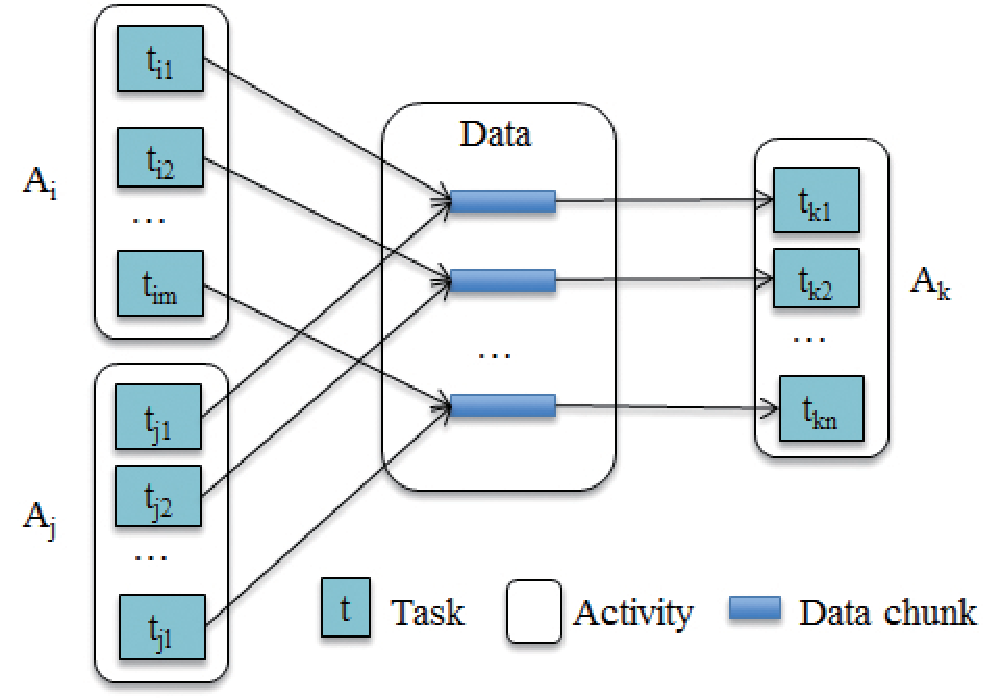
\includegraphics[width=84mm]{figures/SIMD}
\par\end{centering}
\caption{\textbf{Activity and tasks. }}
\label{fig:SIMD}
\end{figure}

\section{Problem Definition}
\label{sec:FGPD}

This section introduces some important terms, \textit{i.e.} SWf and multisite cloud, and formally defines the task scheduling problem we address.

A SWf can be described as a Directed Acyclic Graph (DAG) denoted by $W$($V$,$E$).
Let $V$ = \{$v_1$, $v_2$, ..., $v_n$\} be a set of vertices, which represent the scientific data processing activities. $E$ = \{$e_{i,j}$: $v_i, v_j \in V$ and Activity $v_j$ consumes the output data of Activity $v_i$ \} represents a set of edges that correspond to dependencies between activities in $V$. Activity $v_i$ is the parent activity of Activity $v_j$ and Activity $v_j$ is the child activity of Activity $v_i$.
If it has no parent activity, an activity is a start activity. If it has no child activity, an activity is an end activity. If it has neither parent activity nor child activity, an activity is an intermediate activity. Since an activity may process big amount of data, it corresponds to multiple tasks. Thus, as shown in Figure \ref{fig:SIMD}, an activity $A_k$ may have $n$ tasks \{$t_1$, $t_2$, ..., $t_n$\}, each consuming a data chunk produced by the tasks of parent activities of Activity $A_k$, \textit{i.e.} Activities $A_i$ and $A_j$. A data-intensive SWf is the SWf that it is difficult to manage or transfer data compared to the data processing. For instance, for data-intensive SWfs, the time to transfer data cannot be ignored compared with the time to process data. Different from data-intensive SWfs, the time to transfer data can be ignored for computing-intensive SWfs since it takes much more time to process data compared with the time to transfer data. 


As defined in \cite{Liu2014a}, a multisite cloud is a cloud with multiple distributed data centers of the same cloud provider, each being explicitly accessible to cloud users. A multisite cloud configuration defines the instances of Virtual Machines (VMs) and storage resources for cloud users at a multisite cloud. 
The configured\footnote{Configured for the quota of resources that can be used by a cloud user.} multisite cloud $MS$($S$) consists of a set of cloud sites $S$ with instantiated VMs and data at each site. In this chapter, a cloud site corresponds to a cluster of VMs, data and cloud services, \textit{e.g.} database and message queue service. In the cluster of VMs, each VM is a computing node. 

We assume that the input data of the SWf cannot be moved across different sites. 
Thus, the tasks of the start activity should be scheduled at the site where the data is. 
We assume that the intermediate data can be moved across different sites. 
Thus, the tasks of the intermediate activities or end activities can be scheduled at any site. 
During SWf execution, the tasks of each activity are generated independently and the scheduling of the tasks of each activity is done independently. 
Thus, we need to group tasks of the same activities in bags. Then, a bag of tasks $T$ is a set of tasks corresponding to the same activity.
In addition, we assume that the time to transfer the input data of tasks between two different sites and the time to generate provenance data is non-negligible compared with the execution time of a task.
Scheduling tasks is to choose the sites in $S$ to execute a bag of tasks $T$, \textit{i.e.} mapping each task to an execution site. 
In this chapter, we assume that the input data of the bag of tasks $T$ is distributed at different sites. A scheduling plan defines the mapping of tasks to sites.
Thus, the task scheduling problem is how to generate scheduling plans for a bag of tasks, which corresponds to an activity of a SWf, into sites while reducing the whole execution time of all the tasks in the bag with distributed input data and provenance support. The scheduling process is performed at the beginning of the execution of each activity when the tasks are generated and to be scheduled at each site.


\section{System Design}
\label{sec:FGSA}

\begin{figure}
\begin{centering}
\captionsetup{justification=centering}
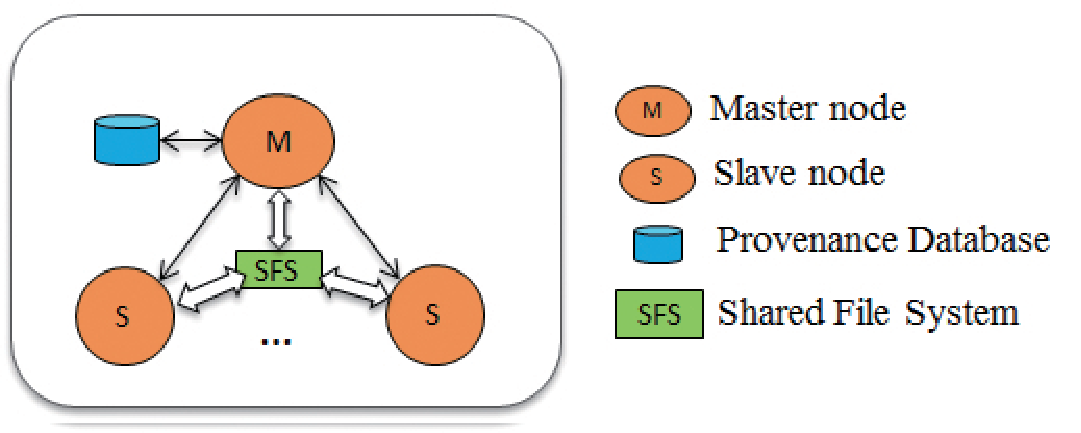
\includegraphics[width=85mm]{figures/EASSC}
\par\end{centering}
\caption{\textbf{Architecture of single site Chiron. }}
\label{fig:EASSC}
\end{figure}

Chiron \cite{Ogasawara2013} is a SWfMS for the execution of data-intensive SWfs at a single site, with provenance support. We adapt Chiron to a multisite cloud environment. In this section, we present the system architecture of single site Chiron and propose the adapted multisite Chiron. 

\subsection{Single Site Chiron}
\label{subsec:SSSA}

At a single site, Chiron takes one computing node as master node and the other nodes as slave nodes, as shown in Figure \ref{fig:EASSC}. In a cloud environment, a computing node is a VM. Designed for HPC environments, Chiron relies on a Shared File System \footnote{In a shared file system, all the computing nodes of the cluster share some data storage that are generally remotely located \cite{Liu2014a}.}, \textit{e.g.} Network File System (NFS) \cite{Sandberg1988}, for managing data. All the computing nodes in the cluster can read or write the data stored in the shared file system.
Chiron exploits a relational database, \textit{e.g.} PosgreSQL, to store provenance data.
 

\begin{figure}
\begin{centering}
\captionsetup{justification=centering}
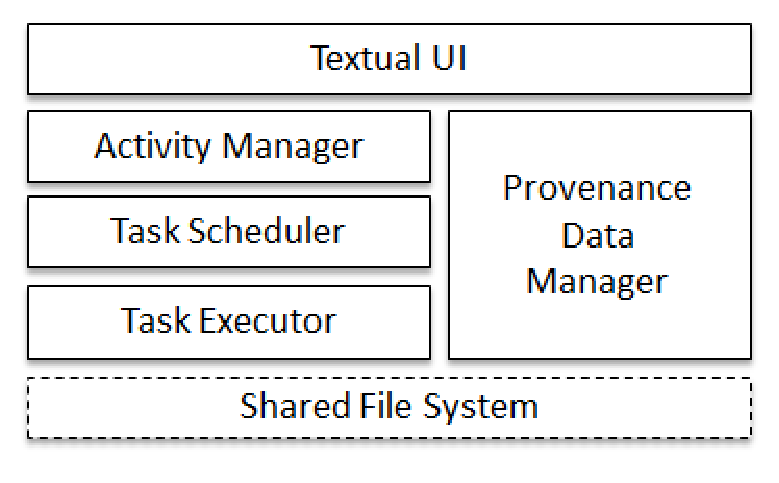
\includegraphics[width=84mm]{figures/CA}
\par\end{centering}
\caption{\textbf{Layered Architecture of Single Site Chiron. } Dashed box, \textit{i.e.} shared file system, represents that the module exploits an external system, \textit{e.g.} NFS, to realize the function.}
\label{fig:CA}
\end{figure}


The layered architecture of single site Chiron is illustrated in Figure \ref{fig:CA}. There are six modules, \textit{i.e.} textual UI, activity manager, single site task scheduler, task executor, provenance data manager and shared file system. 
As for the SWfMS functional architecture presented in Chapter \ref{State}, textual UI corresponds to the presentation layer; provenance data manager corresponds to the user services layer; activity manager and single site task scheduler correspond to the WEP generation layer; task executor is at the WEP execution layer and shared file system is at the infrastructure layer.
The users can use a textual User Interface (UI) to interact with Chiron, in order to start an instance of Chiron at each computing node.
During the execution of a SWf, each activity and its dependencies are analyzed by the activity manager to find executable activities, \textit{i.e.} unexecuted activities, of which the input data is ready.
In order to execute an activity, the corresponding tasks are generated by the activity manager.
Afterwards, the task scheduler schedules each task to a computing node. 
Then, the task execution module at each computing node executes the corresponding scheduled tasks.
When all the tasks of the executable activity are executed, the activity manager analyzes the activities to find new executable activities to execute. The process of activity analysis, task scheduling and task execution are repeated until all activities have been executed.
Since the input data, intermediate data and output data of SWfs are stored in a shared file system, Chiron does not need to manage data transfer between different computing nodes.
During SWf execution, the activity manager, the task scheduler and the task executor generate provenance data, which is gathered by the provenance data manager. The provenance data manager is located at the master node of the cluster.

The single site provenance model \cite{Ogasawara2013} is shown in Figure \ref{fig:SProv}. In this model, a SWf is composed of several activities. An activity has an operator, \textit{i.e.} the program for this activity. The status of the activity can be ready, running or finished. The $activationCommand$ of an activity is to execute the activity. The $extractorCommand$ is to generate provenance data for the corresponding tasks.
The time at which the activity execution starts is $executionStart$ and the time at which it ends is $executionEnd$.
One activity is related to several tasks, input relations and output relations. One relation is the input or output parameters for the activity. Each relation has its own attributes and tuples. The tasks of an activity are generated based on the input relation of the activity. A task processes the files associated with the corresponding activity. Each task has a status, \textit{i.e.} ready, running or finished. In addition, the start time and end time of its execution is recorded as $ExecutionStart$ and $ExecutionEnd$. During execution, the corresponding information of activities, files and tasks are stored as provenance data.

\begin{figure}
\begin{centering}
\captionsetup{justification=centering}
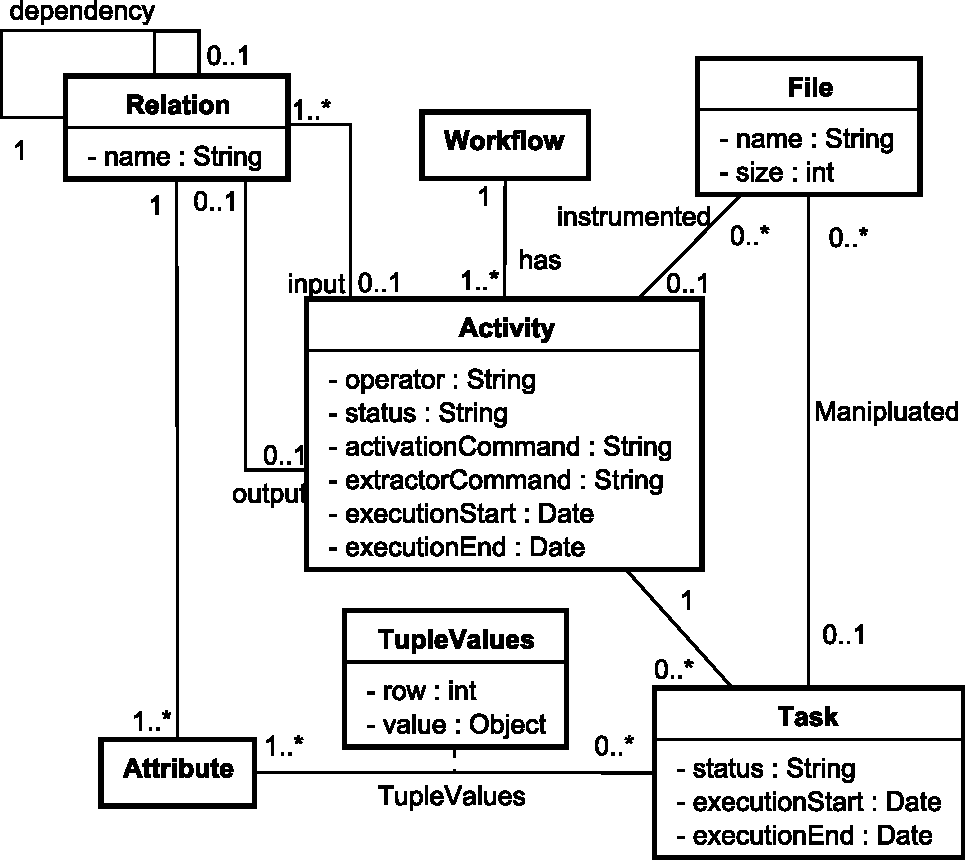
\includegraphics[width=80mm]{figures/SProv}
\par\end{centering}
\caption{\textbf{Single Site Provenance Model \cite{Ogasawara2013}. }}
\label{fig:SProv}
\end{figure}
 
\subsection{Multisite Chiron}
\label{subsec:MSA}

In this section, we present the distributed architecture of multisite Chiron, with the modifications to adapt the single site Chiron to a multisite Cloud.

\begin{figure}
\begin{centering}
\captionsetup{justification=centering}
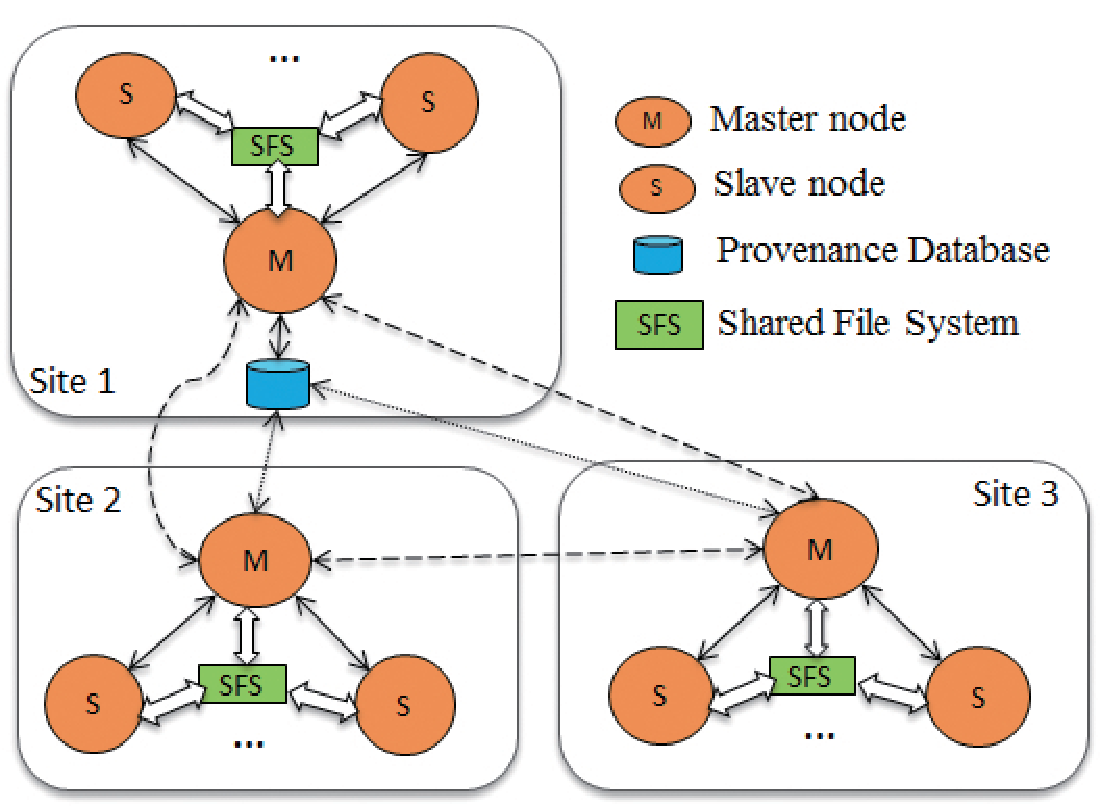
\includegraphics[width=85mm]{figures/MEE}
\par\end{centering}
\caption{\textbf{Architecture of multisite Chiron. }}
\label{fig:MEE}
\end{figure}

In the execution environment of multisite Chiron, there is a master site (site $1$ in Figure \ref{fig:MEE}) and several slave sites (Sites $2$ and $3$ in Figure \ref{fig:MEE}). The master site is similar to the execution environment of a single site Chiron with computing nodes, shared file system and a provenance database. Moreover, a queuing service (see Section \ref{subsec:MCC}) is deployed at the master site. A slave site is composed of a cluster of VMs with a deployed shared file system. In addition, the master node of each site is configured to open the corresponding endpoints to enable the message communication and data transfer with other sites.
In the cloud, an endpoint is a data communication tunnel, which maps a public port of a Web domain to a private port of a computing node within the Web domain. In this chapter, we assume that there is a Web domain at a cloud site, which is used for SWf execution and that all the resources related to SWf execution are in the Web domain at that site. A public port is accessible to all the devices on the Internet. A private port can only be recognized by the devices within the same Web domain. The endpoints can be configured by a user of the cloud.

The layered architecture of multisite Chiron is depicted in Figure \ref{fig:MCA}. The textual UI is present at each node of each site to start an instance of Chiron. The activity manager is located at the master node of the master site to analyze the activities to find executable activities. The multisite task scheduler is also located at the master node of the master site, which schedules the tasks to be executed. The provenance data manager works at the master node of each site to gather provenance data for the tasks executed at each site and updates the provenance data in the provenance database. The task executor is present at each node of each site to execute tasks. The shared file system is deployed at the master node of each site and is accessible to all the nodes of the same site. The multisite file transfer and multisite message communication (corresponding to the infrastructure layer presented in Chapter \ref{State}) work at the master node of each site to enable the communication of different sites.

\begin{figure}
\begin{centering}
\captionsetup{justification=centering}
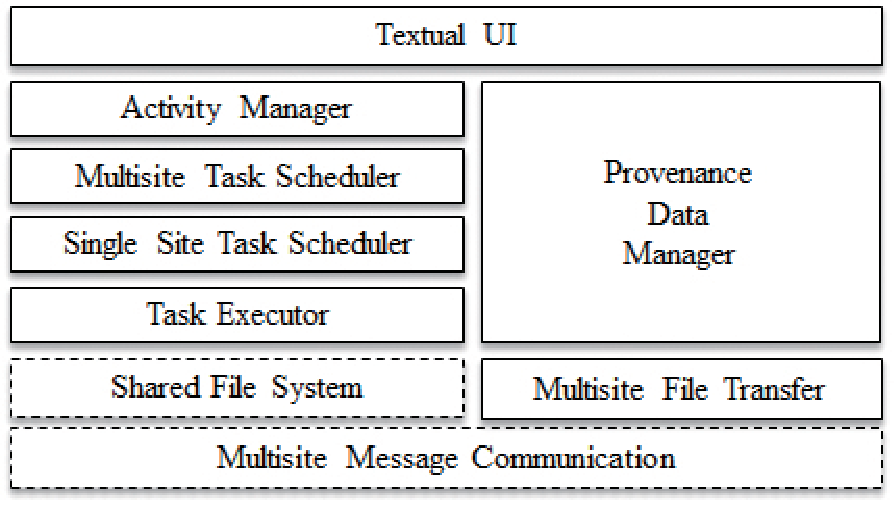
\includegraphics[width=84mm]{figures/MCA}
\par\end{centering}
\caption{\textbf{Multisite layered Architecture. }}
\label{fig:MCA}
\end{figure} 

In order to extend Chiron to a multisite environment, three key aspects, i.e. provenance model, multisite communication and multisite scheduling, must be considered.
First, we adapt the provenance model to the multisite environment. As shown in Figure \ref{fig:MProv}, we add the information about site and computing node (VM) into the provenance model. A site has its own public IP address, public ports for the communication with other sites, number of virtual CPUs, bandwidth to transfer data to the provenance database and bandwidth to transfer data to other sites. A site can contain several VMs. Each VM has its private IP address (which can only be recognized by the devices deployed in the same Web domain), the type of VM, and the number of virtual CPUs. The type of a VM is configured by a cloud user. In a multisite environment, the provenance database is located at a master site. Since one task is executed at one computing node of a specific site, a task is related to one computing node and one site. A file can be stored at several sites. Since the input data of a task may be stored at one site (site $s_1$) and processed at another site (site $s_2$), it is transferred from $s_1$ to $s_2$ before being processed. As a result, the data ends up being stored at the two sites. Thus, one file is related to several sites. In addition, the provenance data can provide data location information for the scheduling process. Thus, users can also get execution information, \textit{i.e.} which task is executed at which site, from the provenance database. The other objects and relationships remain the same as in the single site provenance model.

Second, to support communication between different sites, we add two modules, \textit{i.e.} multisite message communication module and multisite file transfer module. The multisite message communication module is responsible for the exchange of control messages among different sites. The control messages are generated for synchronizing the execution of each site and sharing information among different sites. The multisite file transfer module transfers files to be processed by a task from the site where the files are stored to the site where the task is executed.
The implementation techniques of the two modules are detailed in Section \ref{subsec:MCC}.

\begin{figure}
\begin{centering}
\captionsetup{justification=centering}
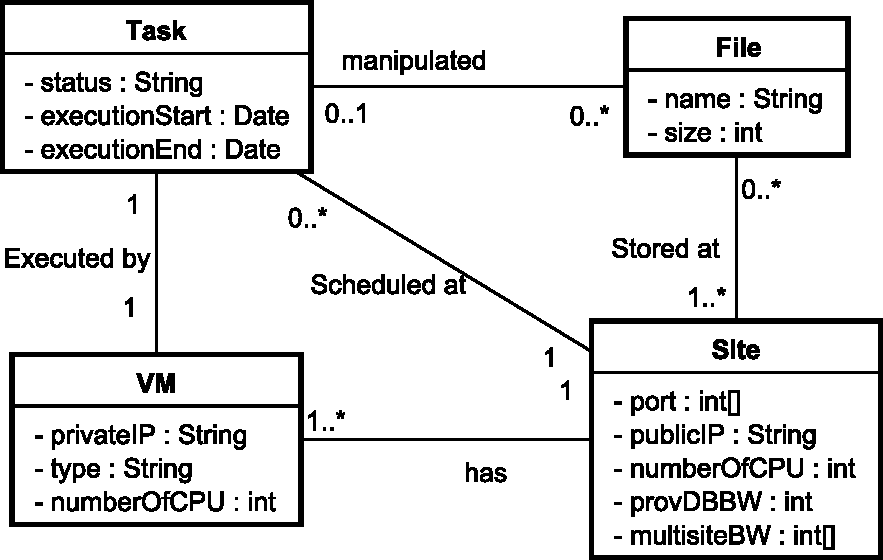
\includegraphics[width=84mm]{figures/MProv}
\par\end{centering}
\caption{\textbf{Multisite Provenance Model.}}
\label{fig:MProv}
\end{figure}

Third, we provide a multisite task scheduling module in multisite Chiron, which is detailed in Section \ref{subsec:MSTS}. 

\section{Task Scheduling}
\label{sec:FGTS}

In this section, we present how single site task scheduling is done in Chiron and propose a multisite task scheduling algorithm, \textit{i.e.} Data-Intensive Multisite task scheduling
(DIM). Then, we analyze the complexity of the DIM algorithm. Finally, we present the method to estimate the execution time of a bag of tasks at a single site cloud, which is used in the DIM algorithm.

\subsection{Single Site Task Scheduling}
\label{subsec:SSTS}

Currently, task scheduling in the single site implementation of Chiron is carried out in a simple way. Tasks are generated and published to a centralized provenance database. Each time a slave node is available, it requests new tasks from the master node, which in turn searches for unexecuted tasks and dispatches them to the slave. This approach is efficient for single site implementations, where communication latency is negligible and there exists an underlying shared file system. 
However, in multisite environments, scheduling has to be carefully performed to avoid costly and unnecessary intersite data transfers and to achieve good load balancing among  sites. 
In a multisite environment, the different data transfer rates between different sites and computing resources should be considered to generate a good scheduling plan. 

\subsection{Multisite Task Scheduling}
\label{subsec:MSTS}

In this section, we propose our mutlisite scheduling algorithm, \textit{i.e.} DIM.
Multisite task scheduling is done with a two Level ($2$L) approach, which is shown in Figure \ref{fig:MS}. The first level performs multisite scheduling, where each task is scheduled to a site. Then, the second level performs single site scheduling, where each task is scheduled to a computing 
\begin{figure}
\begin{centering}
\captionsetup{justification=centering}
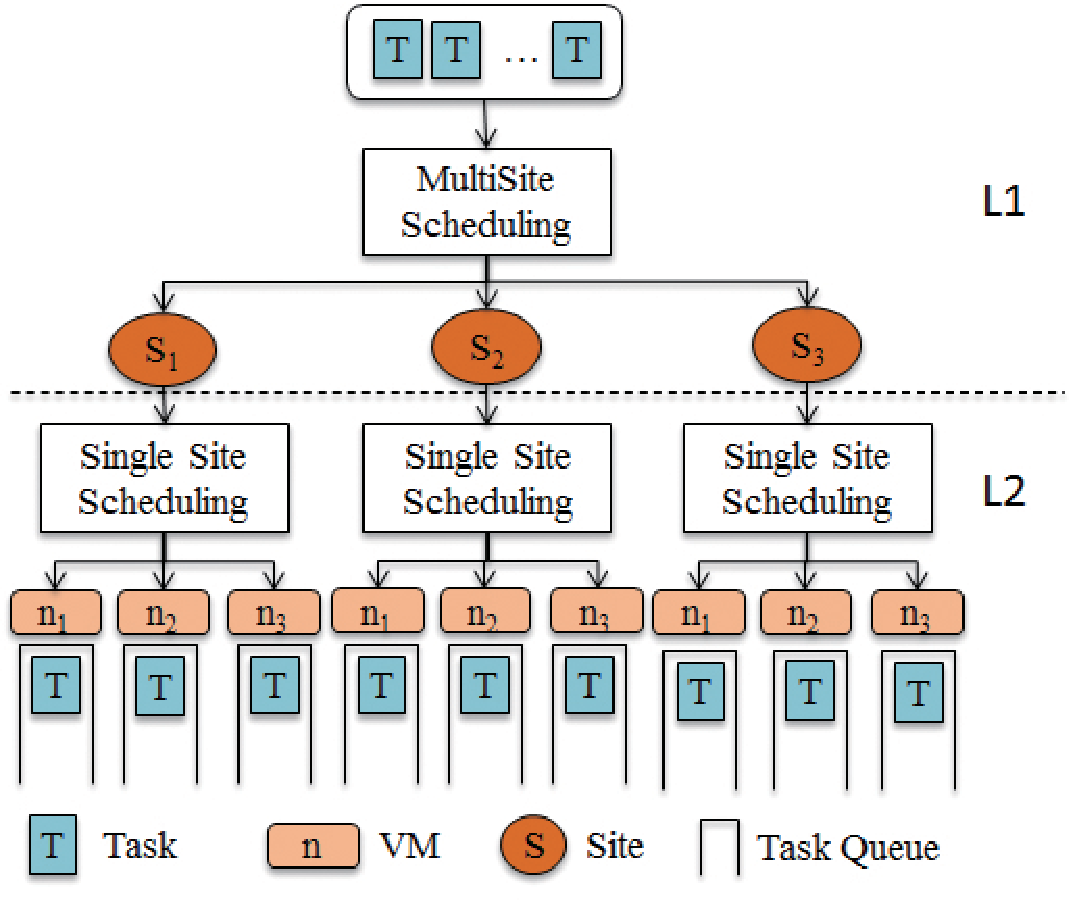
\includegraphics[width=85mm]{figures/MS}
\par\end{centering}
\caption{\textbf{MultiSite Scheduling.} The master node at the master site schedules tasks to each site. At each site, the master node schedules tasks to slave nodes. }
\label{fig:MS}
\end{figure}
\noindent node of the site. 
Compared with a one Level ($1$L) approach that schedules tasks directly to computing nodes at different cloud sites, this $2$L approach may well reduce the multisite scheduling complexity. 
For instance, let us schedule $N$ ($N>>2$) tasks to $M$ ($M>2$) sites, each of which has $K$ ($K>2$) computing nodes. The complexity of the $2$L approach is $M^N + K^N$, where $M^N$ is the complexity of the multisite level and $K^N$ is the complexity of the single site level. Assume that there are $N_i$ tasks scheduled at site $s_i$ while $\sum_{i = 1}^{M}{N_i} = N$. Thus, the complexity of single site scheduling is:
\begin{equation}\label{equ:0}
\begin{split}
\prod_{i = 1}^{M}{K^{N_i}} =& K^{\sum_{i = 1}^{M}{N_i}} \\=& K^N
\end{split}
\end{equation}
Thus, the complexity of the single site scheduling of $2$L approach is $K^N$.
However, the complexity of the $1$L approach is ${(M * K)}^N$. 
Let us assume that $N > 2, M > 2$ and $K > 2$.
\begin{equation}\label{equ:0}
\begin{split}
M^N + K^N <& ~{(\frac{1}{2} * M * K)}^N + {(\frac{1}{2} * M * K)}^N \\
<& ~{(\frac{1}{2})}^{(N - 1)} * {(M * K)}^N \\
<& ~{(M * K)}^N
\end{split}
\end{equation}
From Formula \ref{equ:0}, we can conclude that $N^M + N^K < N^{M * K}$, \textit{i.e.} the complexity of $2$L scheduling approach is smaller than that of $1$L scheduling approach.
In addition, the $2$L scheduling approach can exploit the existing scheduling solutions of single site SWfMSs. 
In this chapter, we focus on the multisite scheduling part, since we use the default scheduling solutions of Chiron for single site scheduling.

In our layered architecture (see Section \ref{subsec:MSA}), the multisite scheduling is performed at the master node of the master site. For the tasks of data-intensive SWfs,  the time to transfer task input data and the time to generate provenance data should not be ignored, in particular in case of low  bandwidth of intersite connection and big amounts of data in the files to be transferred between different sites. This is why we consider the time to transfer task input data and provenance data in the scheduling process. The method to estimate the execution time of a bag of tasks at a single site is detailed in Section \ref{subsec:ETE}. In addition, during the scheduling, if the data cannot be moved, the associated tasks are scheduled at the site where the data is stored.

The DIM algorithm schedules a bag of tasks onto multiple sites (see Algorithm \ref{alg:DIMTS}). First, the tasks are scheduled according to the location of input data (Lines $2$-$5$), which is similar to the scheduling algorithm of MapReduce \cite{Dean2004}.
Line $3$ searches the site that stores the biggest part of input data corresponding to Task $t$. Line $4$ schedules Task $t$ at Site $s$. Line $5$ estimates the execution time of all the tasks scheduled at Site $s$ according to Formula \ref{equ:2}.
Then, the execution time at each site is balanced by adjusting the whole bag of tasks scheduled at that site (Lines $6$-$9$). Line $6$ checks if the maximum difference of the estimated execution time of tasks at each site can be reduced by verifying if the difference is reduced in the previous loop or if this is the first loop.
While the maximum difference of execution time can be reduced, the tasks of the two sites are exchanged as described in Lines $7$-$9$. Line $7$ and $8$ choose the site that has the minimal execution time and the site that has the maximum execution time, respectively. Then, the scheduler calls the function $ExchangeTasks$ to exchange the tasks scheduled at the two selected sites to reduce the maximum difference of execution time. 

\linespread{1.0}
\begin{algorithm}
\caption{Data-Intensive Multisite task scheduling (DIM)}\label{alg:DIMTS}
\begin{algorithmic}[1]
\INPUT $T$: a bag of tasks to be scheduled; $S$: a set of cloud sites
\OUTPUT $SP$: the scheduling plan for $T$ in $S$
\State $SP\gets \emptyset$
\ForAll{$t\in T$}
\State $s\gets GetDataSite( t )$  
\State $SP \gets SP \cup \{ Schedule(t, s) \}$
\State EstimateTime( $T$, $s$, $SP$ )
\EndFor
\While{MaxunbalanceTime( $T$, $s$, $SP$ ) can be reduced}
\State $sMin <- MinTime(S)$ 
\State $sMax <- MaxTime(S)$ 
\State ExchangeTasks($sMin$, $sMax$, $SP$) 
\EndWhile
\ENDBEGIN
\end{algorithmic}
\end{algorithm}

In order to achieve load balancing of two sites, we propose $ExchangeTasks$ algorithm. Let us assume that there are two sites, \textit{i.e.} Sites $s_i$ and $s_j$. For the tasks scheduled at each site, we assume that the execution time of Site $s_i$ is bigger than Site $s_j$. In order to balance the execution time at Sites $s_i$ and $s_j$, some of the tasks scheduled at Site $s_i$ should be rescheduled at Site $s_j$. Algorithm \ref{alg:ET} gives the method to reschedule a bag of tasks from Site $s_i$ to Site $s_j$ in order to balance the load between the two sites. Line $1$ calculates the difference of the execution time of two sites according to Formula \ref{equ:2} with a scheduling plan. Line $2$ gets all the tasks scheduled at Site $s_i$. For each Task $t$ in $T_i$ (Line $3$), it is rescheduled at Site $s_j$ if the difference of execution time of the two sites can be reduced (Lines $4$-$8$). Line $4$ reschedules Task $t$ at Site $s_j$. Line $5$ calculates the execution time at Sites $s_i$ and $s_j$. Lines $6$-$7$ updates the scheduling plan if it can reduce the difference of execution time of the two sites by rescheduling Task $t$. 


\begin{algorithm}
\caption{Exchange Tasks}\label{alg:ET}
\begin{algorithmic}[1]
\INPUT $s_i$: a site that has bigger execution time for its scheduled tasks; $s_j$: a site that has smaller execution time for its scheduled tasks; $SP$: original scheduling plan for a bag of tasks $T$
\OUTPUT $SP$: modified scheduling plan
\State $Diff \gets CalculateExecTimeDiff( s_i, s_j, SP )  $
\State $T_i\gets GetScheduledTasks( s_i, SP )$
\ForAll{$t\in T_i$}
\State $SP' \gets ModifySchedule( SP, \{Schedule(t, s_j)\}$ 
\State $Diff' \gets CalculateExecTimeDiff( s_i, s_j, SP' ) $
\If{$Diff' < Diff$}
\State $SP\gets SP'$
\State $Diff\gets Diff'$
\EndIf
\EndFor
\ENDBEGIN
\end{algorithmic}
\end{algorithm}

\subsection{Complexity}

In this section, we analyze the complexity of the DIM algorithm. 
Let us assume that we have $n$ tasks to be scheduled at $m$ sites. 
The complexity of the first loop (lines $2$-$5$) of the DIM algorithm is $\mathcal{O}(n)$.
The complexity of the $ExchangeTasks$ algorithm is $\mathcal{O}(n)$, since there may be $n$ tasks scheduled at a site in the first loop (lines $2$-$5$) of the DIM algorithm. 
Assume that the difference between the maximum execution time and the minimum execution time is $T_{diff}$.
The maximum value of $T_{diff}$ can be $n * avg(T)$ when all the tasks are scheduled at one site while there is no task scheduled at other sites. $avg(T)$ represents the average execution time of each task, which is a constant value.
After $m$ times of exchanging tasks between the site of maximum execution time and the site of minimum execution time, the maximum difference of execution time of any two sites should be reduced to less than $\frac{T_{diff}}{2}$. 
Thus, the complexity of the second loop (lines $6$-$9$) of the DIM algorithm is $\mathcal{O}(m\cdot n\cdot \log{}n)$.
Therefore, the complexity of the DIM algorithm is $\mathcal{O}(m\cdot n\cdot \log{}n)$. 
It is only a little bit higher than that of OLB and MCT, which is $\mathcal{O}(m\cdot n)$, but yields high reduction in SWf execution (see Section \ref{subsec:exp}).

\subsection{Execution Time Estimation}
\label{subsec:ETE}
We now give the method to estimate the execution time of a bag of tasks at a single site, which is used in both the DIM algorithm and the MCT algorithm.
Formula \ref{equ:21} gives the estimation of execution time without considering the time to generate provenance data, which is used in the MCT algorithm.
\begin{equation}\label{equ:21}
\begin{split}
TotalTime( T, s ) = & ExecTime( T, s ) \\
&+ InputTransTime( T, s ) 
\end{split}
\end{equation}
$T$ represents the bag of tasks scheduled at site $s$. $ExecTime$ is the time to execute the bag of tasks $T$ at site $s$, \textit{i.e.} the time to run the corresponding programs. $InputTransTime$ is the time to transfer the input data of the tasks from other sites to site $s$. 
In the DIM algorithm, we use Formula \ref{equ:2} to estimate the execution time with the consideration of the time to generate provenance data.
\begin{equation}\label{equ:2}
\begin{split}
TotalTime( T, s ) = & ExecTime( T, s ) \\
&+ InputTransTime( T, s ) \\
&+ ProvTransTime( T, s )
\end{split}
\end{equation}
$ProvTransTime$ is the time to generate provenance data in the provenance database. 

We assume that the workload of each task of the same activity is similar. The average workload (in GFLOP) of the tasks of each activity and the computing capacity of each VM at Site $s$ is known to the system. The computing capacity (in GFLOPS) indicates the workload that can be realized per second. Then, the time to execute the tasks can be estimated by dividing the total workload by the total computing capacity of Site $s$, as shown in Formula \ref{equ:3}.
\begin{equation}\label{equ:3}
\begin{split}
ExecTime( T, s ) = \frac{|T| * AvgWorkload( T )}{\sum_{VM_i \in s}ComputingCapacity( VM_i )} 
\end{split}
\end{equation}
$|T|$ represents the number of tasks in Bag $T$. $AvgWorkload$ is the average workload of the bag of tasks. 

The time to transfer input data can be estimated as the sum of the time to transfer the input data from other sites to Site $s$ as shown in Formula \ref{equ:4}.
\begin{equation}\label{equ:4}
\begin{split}
InTransTime( T, s ) = \sum_{t_i \in T}\sum_{s_i \in S}\frac{InDataSize( t_i, s_i )}{DataRate( s_i, s )}
\end{split}
\end{equation}
$InDataSize( t_i, s_i)$ represents the size of input data of Task $t_i$, which is stored at Site $s_i$. The size can be measured at runtime. $DataRate( s_i, s )$ represents the data transfer rate, which can be configured by users. $S$ represents the set of sites. 

Finally, the time to generate provenance data is estimated by Formula \ref{equ:5}.
\begin{equation}\label{equ:5}
\begin{split}
ProvTransTime( T, s ) = &|T| * TransctionTimes( T ) \\ & * AvgTransactionTime( s )
\end{split}
\end{equation}
$|T|$ represents the number of tasks in Bag $T$. We can estimate $AvgTransactionTime$ by counting the time to perform a data exchange to update the provenance data of a task in the provenance database from Site $s$. $TransctionTimes( T )$ represents the number of data exchanges to perform for generating the provenance data of each task in Bag $T$. It can be configured according to the features of the SWfMS.

\section{Experimental Evaluation}
\label{sec:FGVal}
In this section, we present an experimental evaluation of our DIM scheduling algorithm using Microsoft Azure multisite cloud \cite{Azure}. First, we present two real-life SWfs, \textit{i.e.} Buzz and Montage, as use cases. Then, we explain the techniques for the implementation of intersite communication of multisite Chiron in Azure. Afterwards, we show the experimental results of executing the two SWfs in Azure with different multisite scheduling algorithms.


\begin{figure}
\begin{centering}
\captionsetup{justification=centering}
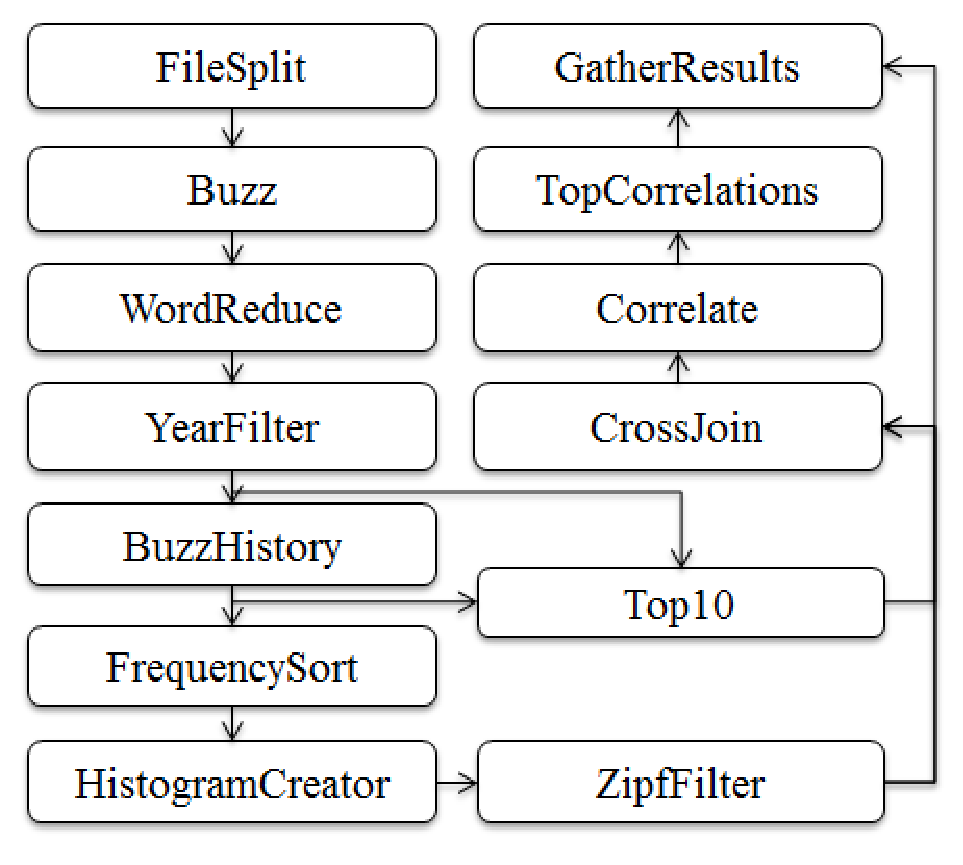
\includegraphics[width=84mm]{figures/Buzz}
\par\end{centering}
\caption{\textbf{Buzz Workflow.}}
\label{fig:buzz}
\end{figure}

\subsection{SWf Use Cases}

In this section, we present two SWfs, \textit{i.e.} Buzz and Montage, to evaluate our proposed algorithms. The two SWfs have different structures, which can show that our proposed algorithm is suitable for different SWfs.

\subsubsection{Buzz Workflow}
Buzz workflow (see Section \ref{sec:UCBuzz} for details) is a data-intensive SWf that searches for trends and measures correlations in scientific publications as shown in Figure \ref{fig:buzz}. 

There are five activities, \textit{i.e.} FileSplit, Buzz, BuzzHistory, HistogramCreator and Correlate, that correspond to multiple tasks. In our experiment, the tasks of the five activities are scheduled by the multisite scheduling algorithm. The other activities exploit a database management system to process data at the master site.

\subsubsection{Montage Workflow}
As presented in Section \ref{subsubsec:SWE}, Montage is a data-intensive SWf for computing mosaics of input images \cite{Deelman2008}.  The input data and the intermediate data are of considerable size and require significant storage resources. However, the execution time of each task is relatively small, which can be at most a few minutes. The structure (at activity level) of the Montage SWf is shown in Figure \ref{fig:montage}. Activity $1$, mProjectPP, reprojects single images to a specific scale. The mDiffFit activity performs a simple image difference between a single pair of overlapping images, which is generate by the mProjectPP activity. Then, the mConcatFit activity gathers the results of mDiffFit into a single file. Afterwards, mBgModel uses the image-to-image difference parameter table to interactively determine a set of corrections to apply to each image to achieve a \textquotedblleft best\textquotedblright ~global fit. The mBackground activity removes a background from a single image. This activity takes the output data of the mProjectPP activity and that of the mBgModel activity. The mImgTbl activity prepares the information for putting the images together. The mAdd activity generates an output mosaic and the binning of the mosaic is changed by the mShrink activity. Finally, the mJPEG activity creates a JPEG image from the mosaic. In addition, Montage can correspond to different square degrees \cite{Deelman2008} (or degree for short), each of which corresponds to a different number of tasks. 

\begin{figure}
\begin{centering}
\captionsetup{justification=centering}
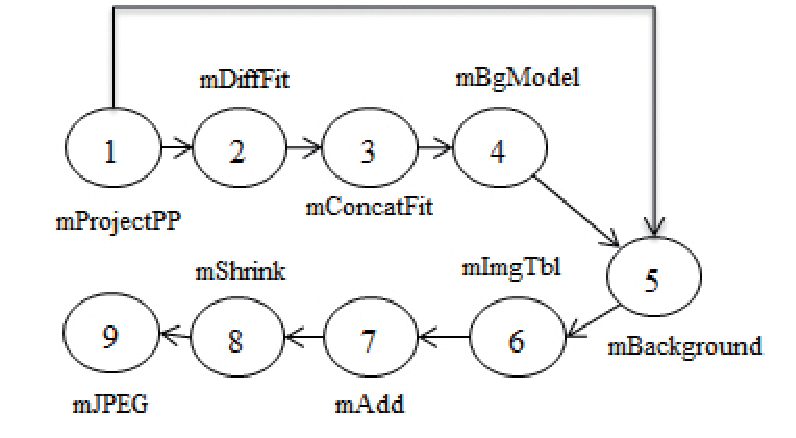
\includegraphics[width=85mm]{figures/Montage}
\par\end{centering}
\caption{\textbf{Montage Workflow.}}
\label{fig:montage}
\end{figure}

\subsection{Intersite Communication}
\label{subsec:MCC}

In this section, we present the detailed techniques for the multisite file transfer module and multisite message communication module.
We choose Azure Service Bus \cite{AzureServiceBus} to realize the functionality of message communication module. Azure Service Bus is a generic, cloud-based messaging system for the communication among different devices. The communication can be based on the HTTP protocol, which does not need to maintain connection information (HTTP is stateless). Although this may bring more overhead for each message, the amount of control messages is low and this cost is negligible. 
The file transfer module is realized by Java TCP connections between two master nodes of two different sites. Since the idle intersite TCP connections may be cut down by the cloud operator, \textit{e.g.} every $5-10$ minutes in Azure, the connections are maintained by sending $keepalive$ messages. For instance, two messages per time period. Before execution, a task is scheduled at a site by the multisite task scheduler. If they are not stored at the scheduled site, the input files of the task are transferred to the scheduled site by the multisite file transfer module.

\subsection{Experiments}
\label{subsec:exp}
This section gives our experimental evaluation of the DIM algorithm, within Microsoft Azure. Azure \cite{Azure} has multiple cloud sites, \textit{e.g.} Central US (CUS), West Europe (WEU) and North Europe (NEU). 
We instantiated three A$4$ (the type of VMs in Azure \cite{AzureVM}) VMs at each of the three site, \textit{i.e.} CUS, WEU and NEU. 
We take WEU as a master site. We deploy an A$2$ VM at WEU and install PostgreSQL database to manage provenance data.
We assume that the input data of the SWfs are distributed at the three sites. 
We compare our proposed algorithm with two representative baseline scheduling algorithms, \textit{i.e.} Opportunistic Load Balancing (OLB) and Minimum Completion Time (MCT). In the multisite environment, OLB randomly selects a site for a task while MCT schedules a task to the site that can finish the execution first. 


\begin{figure}
\begin{centering}
\captionsetup{justification=centering}
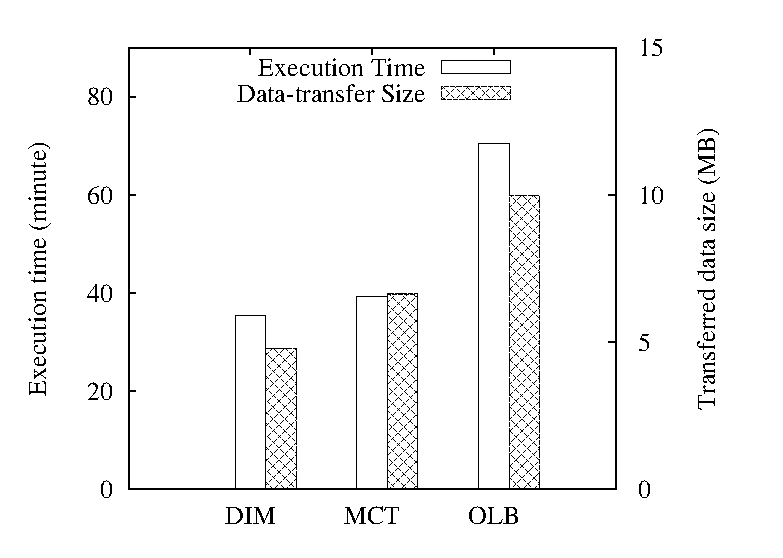
\includegraphics[width=84mm]{figures/60buzz}
\par\end{centering}
\caption{\textbf{Buzz SWf Execution time.} The amount of data is $60$MB.}
\label{fig:Buzz60}
\end{figure}

First, we used a DBLP $2013$ XML file of $60$MB as input data for Buzz SWf in our experiments. The input data is partitioned into three parts, which have almost the same amount of data, and each part is stored at a site while configuration files of Buzz SWf are present at all the three sites. We take WE as a master site. The provenance database and Azure Service Bus are also located at the WE site.
The execution result corresponding to each scheduling algorithm is shown in Figure \ref{fig:Buzz60}. During scheduling, if the data cannot be moved (for the start activity, \textit{i.e.} FileSplit), the associated task is scheduled at the site where the data is stored.

Figure \ref{fig:Buzz60} shows that DIM is much better than MCT and OLB in terms of both execution time and transferred data size. The execution time corresponding to DIM is $9.6\%$ smaller than that corresponding to MCT and $49.6\%$ smaller than that corresponding to OLB. The size of the data transferred between different sites corresponding to MCT is $38.7\%$ bigger than that corresponding to DIM and the size corresponding to OLB is $108.6\%$ bigger than that corresponding to DIM. 

Second, we performed an experiment using a DBLP $2013$ XML file of $1.29$GB as input data for Buzz SWf while configuration files of Buzz SWf are present at all the three sites. The other configuration is the same as the first one. The execution results are shown in Figure \ref{fig:ET}. 

\begin{figure}
\begin{centering}
\captionsetup{justification=centering}
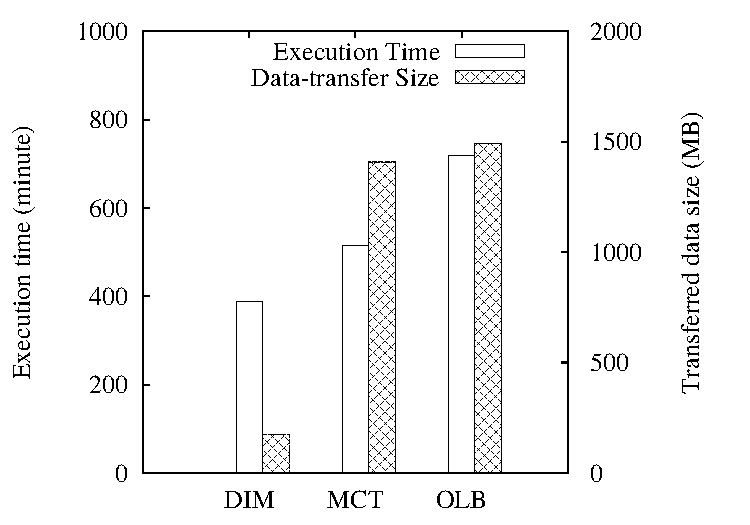
\includegraphics[width=84mm]{figures/execTime}
\par\end{centering}
\caption{\textbf{Buzz SWf Execution time.} The amount of data is $1.29$GB.}
\label{fig:ET}
\end{figure}

Figure \ref{fig:ET} shows that the advantage of DIM in terms of both execution time and transferred data size compared with MCT and OLB increases with bigger amounts of input data. The execution time corresponding to DIM is $24.3\%$ smaller than that corresponding to MCT and $45.9\%$ smaller than that corresponding to OLB. The size of the data transferred between different sites corresponding to MCT is $7.19$ times bigger than that corresponding to DIM and the size corresponding to OLB is $7.67$ times bigger than that corresponding to DIM. 

Since the DIM algorithm considers the time to transfer intersite provenance data and makes optimization for a bag of tasks, it can reduce the data transferred between different sites and the total execution time. MCT only optimizes the load balancing for each task among different sites without consideration of the time to transfer intersite provenance data. It is a greedy algorithm that can reduce the execution time by balancing the execution time of each site while scheduling each task. However, it cannot optimize the scheduling for the whole execution of all the tasks of an activity. In addition, compared with OLB, MCT cannot reduce much the transferred data among different sites. Since OLB simply tries to keep all the sites working on arbitrary tasks, it has the worst performance.

Furthermore, we executed the Montage SWf with $0.5$ degree with three sites, \textit{i.e.} CUS, WEU and NEU. The size of input data is $5.5$GB. The input data is evenly partitioned to three parts stored at the corresponding sites with configuration files stored at all the three sites. The execution time and amount of intersite transferred data corresponding to each scheduling algorithm are shown in Figure \ref{fig:Montage}. 

\begin{figure}
\begin{centering}
\captionsetup{justification=centering}
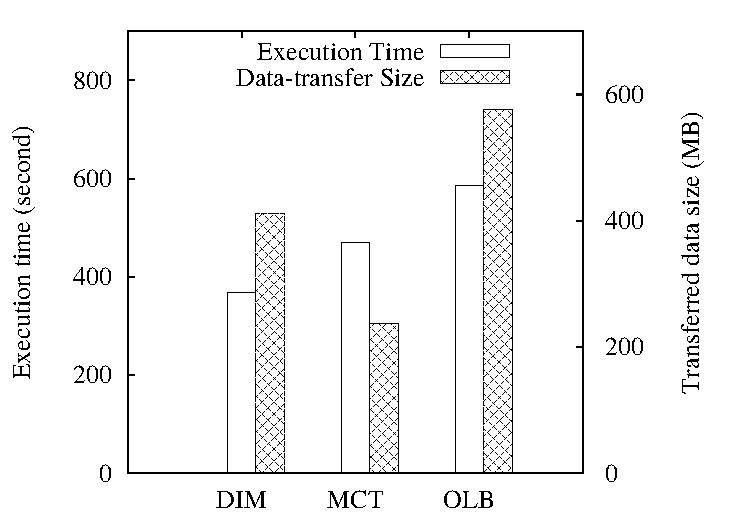
\includegraphics[width=84mm]{figures/montage05}
\par\end{centering}
\caption{\textbf{Montage SWf Execution time.} $0.5$ degree.}
\label{fig:Montage}
\end{figure}

The execution results of Montage with $0.5$ degree reveals that the execution time of DIM is $21.7\%$ smaller than that of MCT and $37.1\%$ smaller than that of OLB. This is expected since DIM makes optimization for a bag of tasks in order to reduce intersite transferred data with consideration of the time to transfer intersite intermediate data and provenance data. MCT is optimized for  load balancing only with consideration of intermediate data. OLB has no optimization for load balancing. In addition, the intersite transferred data of DIM is $42.3\%$ bigger than that of MCT. Since DIM is designed to achieve load balancing of each site to reduce execution time, it may yield more intersite transferred data in order to achieve load balance. However, the amount of intersite transferred data of DIM is $28.6\%$ smaller than that of OLB. This shows the efficiency of the optimization for the data transfer of DIM. Moreover, when the degree ($0.5$) is low, there is less data to be processed by Montage, and the number of tasks to schedule is small. Since DIM is designed for high numbers of tasks, the amounts of intersite transferred data are not reduced very much in this situation.

Finally, we executed Montage SWf of $1$ degree in the multisite cloud. We used the same input data as in the previous experiment, \textit{i.e.} $5.5$GB input data evenly distributed at three sites. The execution time and the amount of intersite transferred data corresponding to each scheduling algorithm are shown in Figure \ref{fig:Montage8}. 

\begin{figure}
\begin{centering}
\captionsetup{justification=centering}
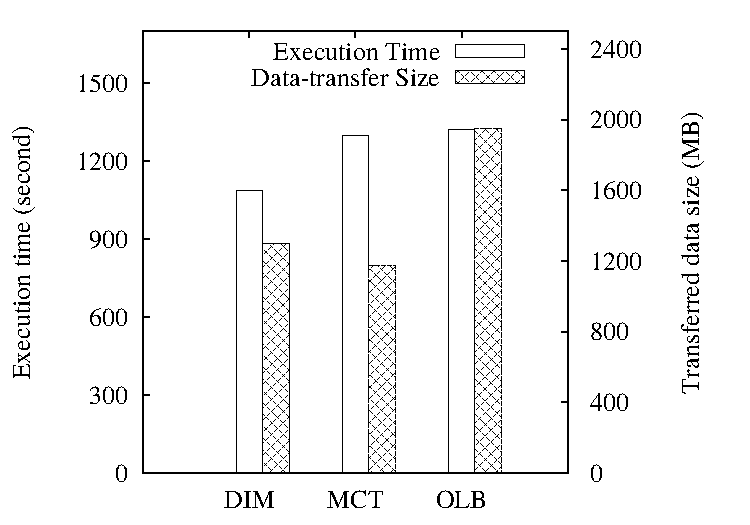
\includegraphics[width=84mm]{figures/montage1}
\par\end{centering}
\caption{\textbf{Montage SWf Execution time.} $1$ degree.}
\label{fig:Montage8}
\end{figure}

The execution results of Montage with $1$ degree reveals that the execution time of DIM is $16.4\%$ smaller than that of MCT and $17.8\%$ smaller than that of OLB. As explained before, this is expected since DIM can reduce the execution time by balancing the load among different sites compared with MCT and OLB. In addition, the intersite transferred data of DIM is $10.7\%$ bigger than that of MCT. This is much smaller than the value for $0.5$ degree ($42.3\%$), since there are more tasks to schedule when the degree is $1$ and DIM reduces intersite transferred data for a big amount of tasks. However, the amount of intersite transferred data is bigger than that of MCT. This happens since the main objective of DIM is to reduce execution time instead of reducing intersite transferred data. In addition, the amount of intersite transferred data of DIM is $33.4\%$ smaller than that of OLB, which shows the efficiency of the optimization for the data transfer of DIM.

\begin{table}[htb]
\caption{\textbf{Scheduling Time. } The unit of time is second. The size of the input data of Buzz SWf is $1.2$GB and the degree of Montage is $1$\protect\footnotemark .}
\label{tab:ST}
\begin{centering}
\captionsetup{justification=centering}
\begin{tabular}{|c|c|c|c|}
\hline 
Algorithm & DIM & MCT & OLB \tabularnewline
\hline 
Buzz & 633 & 109 & 17 \tabularnewline
Montage & 29.2 & 28.8 & 1.5 \tabularnewline
\hline 
\end{tabular}
\par\end{centering} 
\end{table}

In addition, we measured the time to execute the scheduling algorithms to generate scheduling plans while executing Buzz and Montage. The scheduling time is shown in Table \ref{tab:ST}. The complexity of MCT is the same as that of OLB, which is $\mathcal{O}(m\cdot n)$. 
However, the scheduling time of MCT is much bigger than OLB. The reason is that MCT needs to interact with the provenance database to get the information of the files in order to estimate the time to transfer the files among different sites.
The table shows that the time to execute DIM is much higher than OLB for both Buzz and Montage since the complexity of DIM is higher than that of OLB and that DIM has more interactions with the provenance database in order to estimate the execution time of the tasks at a site. When there are significant number of tasks to schedule (for the Buzz SWf), the time to execute DIM is much bigger than that of MCT because of higher complexity.
However, when the number of tasks is not very big, the time to execute DIM is similar to that of MCT. The scheduling time of DIM and MCT is much bigger than that of OLB, since it takes much time to communicate with the provenance database for the estimation of the execution time of each site.
The scheduling time of the three scheduling algorithms is always small compared with the total execution (less than $3$\%), which is acceptable for the task scheduling during SWf execution.
Although the scheduling time of DIM is much bigger than MCT and OLB, the total execution time of SWfs corresponds to DIM is much smaller than that of MCT and OLB as explained in the four experiments. This means that DIM generates better scheduling plans compared with MCT and OLB.

\footnotetext{The advantage of DIM over MCT and OLB is more obvious when the input data of Buzz is $1.2$GB and the degree of Montage is $1$ compared with the other cases in our experiments, \textit{i.e.} when the input data of Buzz is $60$MB and the degree of Montage is $0.5$.}

\begin{table}[htb]
\caption{\textbf{Size of Provenance Data. } The unit of the data is MB. The size of the input data of Buzz SWf is $1.2$GB and the degree of Montage is $1$.}
\label{tab:SPD}
\begin{centering}
\captionsetup{justification=centering}
\begin{tabular}{|c|c|c|c|}
\hline 
Algorithm & DIM & MCT & OLB \tabularnewline
\hline 
Buzz & 301 & 280 & 279 \tabularnewline
Montage & 10 & 10 & 10 \tabularnewline
\hline 
\end{tabular}
\par\end{centering} 
\end{table}


\begin{figure}
\begin{centering}
\captionsetup{justification=centering}
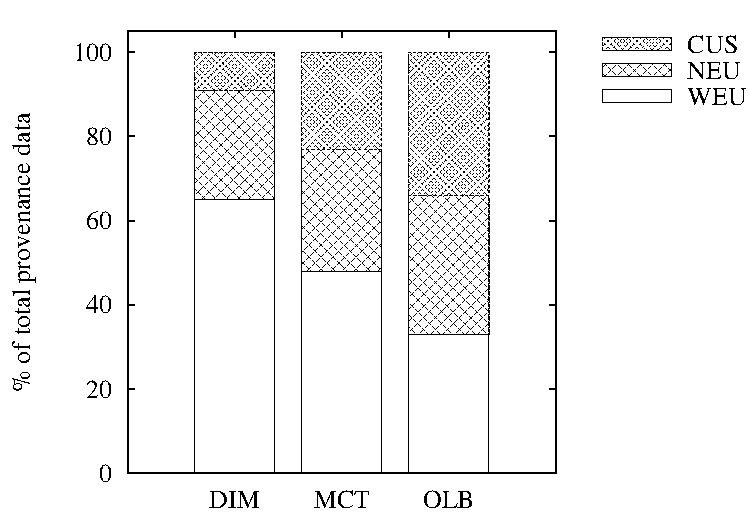
\includegraphics[width=84mm]{figures/provBuzz}
\par\end{centering}
\caption{\textbf{Distribution of provenance during the execution of Buzz workflow.} The size of input data is $1.2$GB.}
\label{fig:provBuzz}
\end{figure}

Furthermore, we measured the size of provenance data and the distribution of the provenance data. As shown in Table \ref{tab:SPD}, the amount of the provenance data corresponding to the three scheduling algorithms are similar (the difference is less than $8\%$). However, the distribution of the provenance data is different. In fact, the bandwidth between the provenance database and the site is in the following order: WEU $>$ NEU $>$ CUS \footnote{For instance, the time to execute "SELECT count(*) from eactivity" at the provenance database from each site: $0.0027$s from WEU site, $0.0253$s from NEU site and $0.1117$s from CUS site.}. As shown in Figures \ref{fig:provBuzz} and \ref{fig:provMontage}, the provenance data generated at CUS site is much more than that generated at NEU site and WEU site for DIM algorithm. In addition, the percentage of provenance data at WEU corresponding to DIM is much bigger than MCT (up to $95\%$ bigger) and OLB (up to $97\%$ bigger). This indicates that DIM can schedule tasks to the site (WEU) that has bigger bandwidth with the provenance database (the database is at WEU site), which yields bigger percentage of provenance data generated at the site. This can reduce the time to generate provenance data in order to reduce the overall multisite execution time of SWfs. However, MCT and OLB is not sensitive to the centralized provenance data, which correspond to bigger multisite execution time.

\begin{figure}
\begin{centering}
\captionsetup{justification=centering}
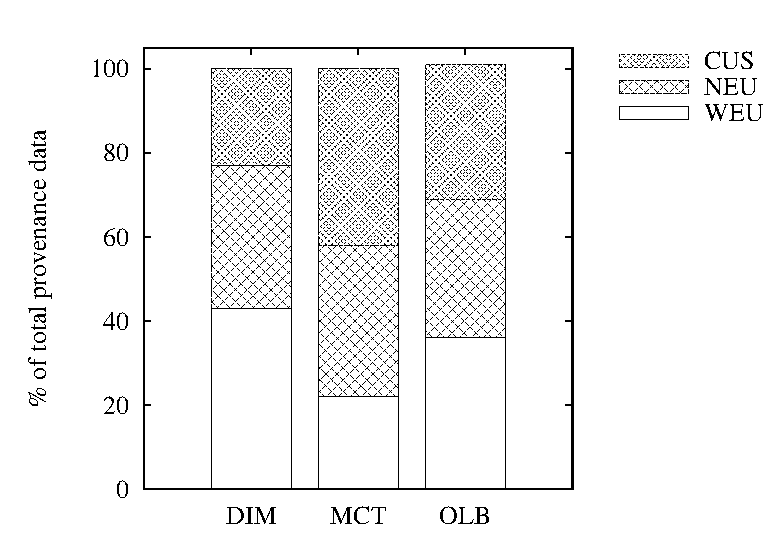
\includegraphics[width=84mm]{figures/provMontage}
\par\end{centering}
\caption{\textbf{Distribution of provenance during the execution of Montage workflow.} The degree is $1$.}
\label{fig:provMontage}
\end{figure}

From the experiments, we can see that DIM performs better than MCT (up to $24.3\%$) and OLB (up to $49.6\%$) in terms of execution time although it takes more time to generate scheduling plans. The scheduling time of MCT is always reasonable compared with the total SWf execution time (less than $3$\%). DIM can reduce the intersite transferred data compared with MCT (up to $719\%$) and OLB (up to $767\%$). As the amount of input data increases, the advantage of DIM becomes more important. 

\section{Conclusion}
\label{sec:FGCon}

Although some SWfMSs with provenance support, \textit{e.g.} Chiron, have been deployed in the cloud, they are generally designed for a single site. In this chapter, we proposed a solution based on multisite Chiron.

Multisite Chiron is able to execute SWfs in a multisite cloud with geographically distributed input data. We proposed the architecture of multisite Chiron, defined a new provenance model for multisite SWf execution and a global method to gather the distributed provenance data in a centralized database. Based on this architecture, we proposed a new scheduling algorithm, \textit{i.e.} DIM, which considers the latency to transfer data and to generate provenance data in multisite cloud. We analyzed the complexity of DIM ($\mathcal{O}(m\cdot n\cdot \log{}n)$), which is quite acceptable for scheduling bags of tasks. We used two real-life SWfs, \textit{i.e.} Buzz and Montage to evaluate the DIM algorithm in Microsoft Azure with three sites. The experiments show that although its complexity is higher than that of OLB and MCT, DIM is much better than two representative baseline algorithms, \textit{i.e.} MCT (up to $24.3\%$) and OLB (up to $49.6\%$), in terms of execution time. In addition, DIM can also reduce significantly data transfer between sites, compared with MCT (up to $719\%$) and OLB (up to $767\%$). Moreover, the scheduling time of MCT is always reasonable compared with the total SWf execution time (less than $3$\%).  The advantage of DIM becomes important with high numbers of tasks.
